%!TEX program = xelatex
\documentclass[24pt]{beamer}
\usepackage[utf8]{inputenc}
\usepackage{xeCJK}
\setCJKmainfont{[simhei.ttf]}
\usepackage{fontspec}
\usepackage{listings}
\usepackage{blindtext}
\usepackage{graphicx}
\usepackage{algorithm2e}

\usetheme{Execushares}

%------------------------------------------------------------
\title{计算机视觉:人脸识别}
\subtitle{https://github.com/yangminz/tensorface}
\author{赵阳旻,14307130067}
\date{2016 12}

\setcounter{showSlideNumbers}{1}

\begin{document}
\setcounter{showProgressBar}{0}
\setcounter{showSlideNumbers}{0}

\frame{\titlepage}
%------------------------------------------------------------
\begin{frame}
\frametitle{目录}
\begin{enumerate}
\item 人脸识别介绍 \\ \textcolor{ExecusharesGrey}{\footnotesize\hspace{1em} 从FBI的文章开始}
\item 卷积神经网络  \\ \textcolor{ExecusharesGrey}{\footnotesize\hspace{1em} 一点点深度的学习}
\item 主成分分析  \\ \textcolor{ExecusharesGrey}{\footnotesize\hspace{1em} 精彩又典雅的传统数学方法}
\item 总结 \\ \textcolor{ExecusharesGrey}{\footnotesize\hspace{1em} 人脸识别:一项既成熟又不成熟的技术}
\end{enumerate}
\end{frame}
%------------------------------------------------------------
\setcounter{framenumber}{0}
\setcounter{showProgressBar}{1}
\setcounter{showSlideNumbers}{1}
\section{人脸识别介绍}
\begin{frame}
\frametitle{当然应用是非常广泛的}
静态照片的人脸识别应用已经很广泛了,毋论动态视频中的识别\\
\begin{center}
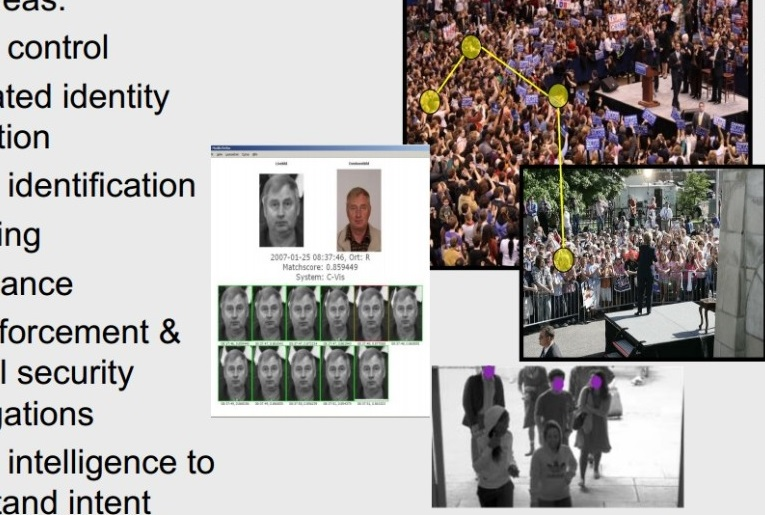
\includegraphics[width=0.6\linewidth]{fig05.jpg}
\end{center}
FBI在某次枪击案中使用了人脸识别技术,从在场人群手机上的和监控中的照片里找到了凶手
\end{frame}
%------------------------------------------------------------
\begin{frame}
\frametitle{简单的历史回顾}
\begin{itemize}
\item 1960s,计算图片上眼耳鼻特征的距离和比例,然后和参考值比较
\item 1970s,使用发色、唇厚等进行自动计算
\item 1988, PCA的应用横空出世,一个milestone
\item 1991, 利用eigenface的残差误差建立实时系统
\item now, CNN大行其道
\end{itemize}
\end{frame}
%------------------------------------------------------------
\section{卷积神经网络}
\begin{frame}
\frametitle{卷积不卷积}
数学上独立随机变量$\xi$与$\eta$的离散卷积是:
\[ P\{\zeta = r\} = \sum_{k = 0}^r P\{ \xi=k, \eta=r-k \} = \sum_{k = 0}^r a_k b_{r - k} \]
CNN的卷积是:
\begin{center}
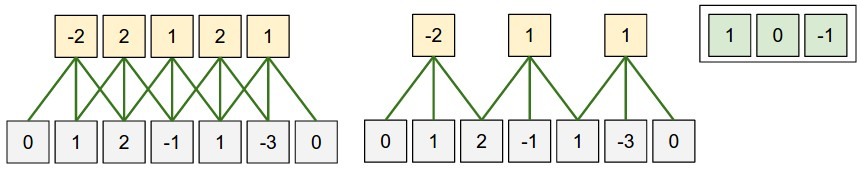
\includegraphics[width=0.8\linewidth]{fig09.jpg}
\end{center}
它只是局部加权平均
\end{frame}
%------------------------------------------------------------
\begin{frame}
\frametitle{来自CS231N的网络}
\begin{center}
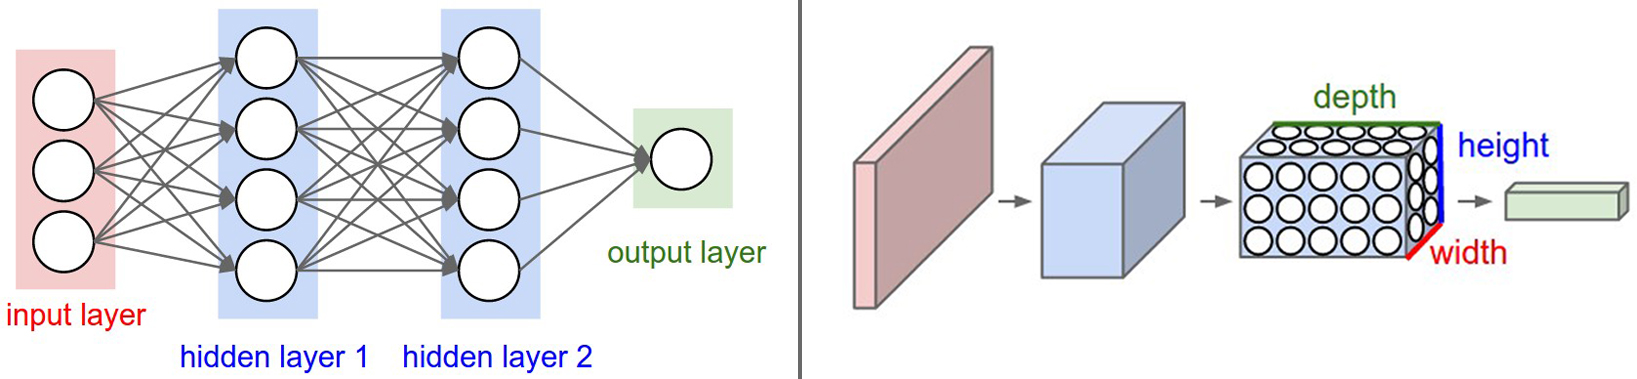
\includegraphics[width=0.9\linewidth]{fig10.jpg}
\end{center}
左边是3层全连接神经网络,右边是一个卷积神经网\\
CNN在于,对于复杂的输入——图片,大量地减少了网络参数的数量
\end{frame}
%------------------------------------------------------------
\begin{frame}
\frametitle{来自CS231N的网络}
与一般网络的差别:
\begin{center}
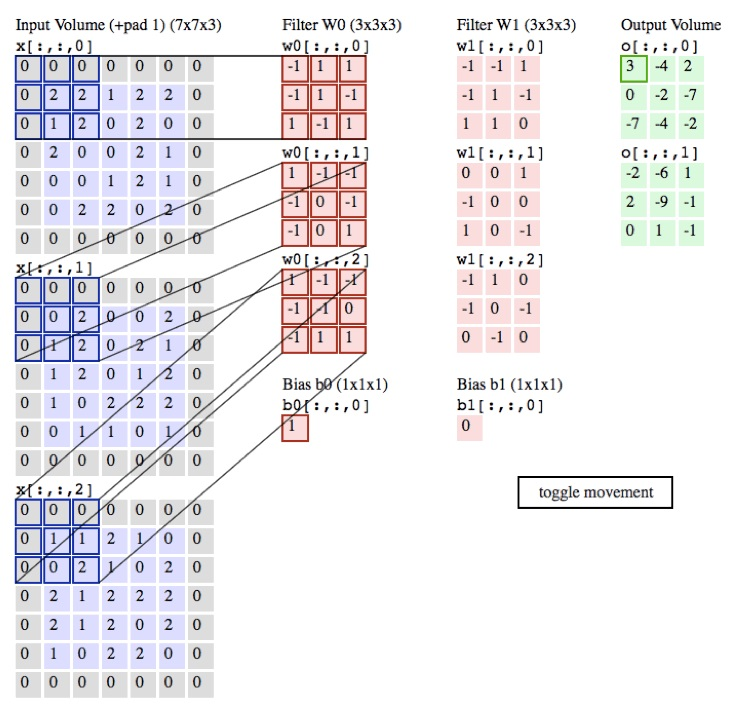
\includegraphics[width=0.47\linewidth]{fig11.jpg}
\end{center}
带来的问题是,虽然CNN通过卷积有效地减少了网络参数\\
但是相比于一般网络,它为什么仍然能够有效?
\end{frame}
%------------------------------------------------------------
\begin{frame}
\frametitle{Kolmogorov定理}
$\Phi (y)$是单调有界连续增函数,其中$y = f(x_1, x_2, \ldots, x_n)$只是一个有界闭子集上的连续函数,则:\\
$\forall \epsilon > 0$,存在正整数$H$和$c_j, \theta_j$,有$w_{ij},i,j \in \{ 1,2,\ldots,n\}$,
\[ g(x_1,x_2,\ldots,x_n) = \sum_{j=1}^H c_j \Phi \left( \sum_{i=1}^n w_{ij} \cdot x_i - \theta_j \right) \]
\[ s.t. \max |f(x_1,x_2,\ldots,x_n) - g(x_1,x_2,\ldots,x_n)| < \epsilon\]
$\Phi(\cdot)$是我们平时用的非线性函数,$c,w,\theta$是随机梯度训练的参数\\
CNN修改了$w$,让函数逼近收敛得更快
\end{frame}
%------------------------------------------------------------
\begin{frame}
\frametitle{一种玄学的解释}
局部感知
\begin{center}
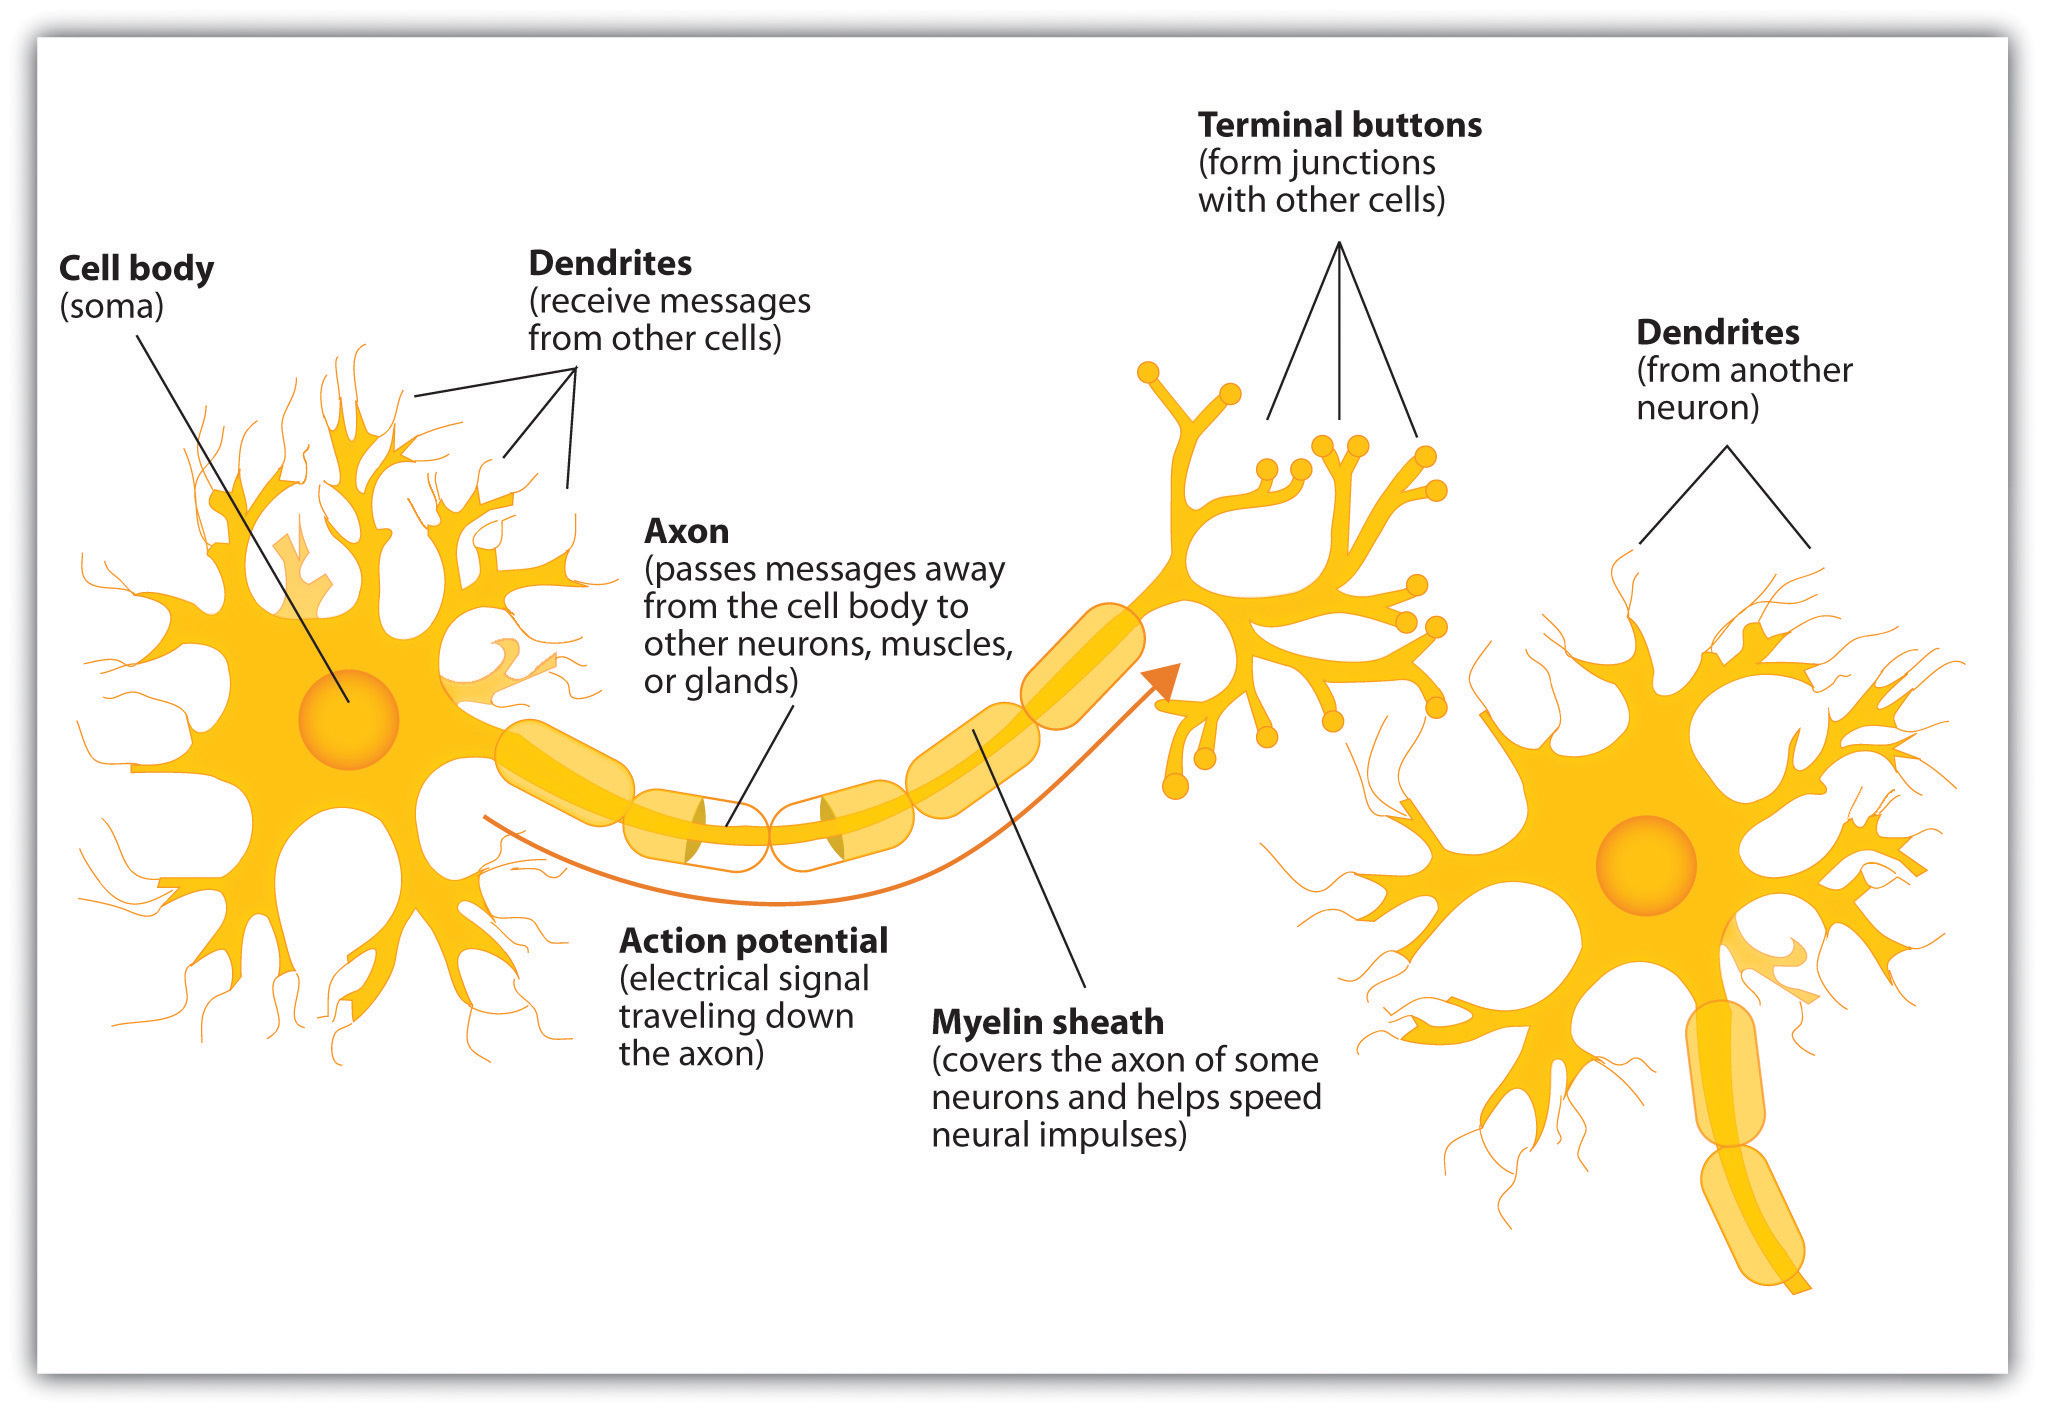
\includegraphics[width=0.7\linewidth]{fig12.jpg}
\end{center}
因为人类的神经元也只具有局部感知能力
\end{frame}
%------------------------------------------------------------
\begin{frame}
\frametitle{Keras实验:实际上发生了什么}
使用AT\&T的数据集:
\begin{center}
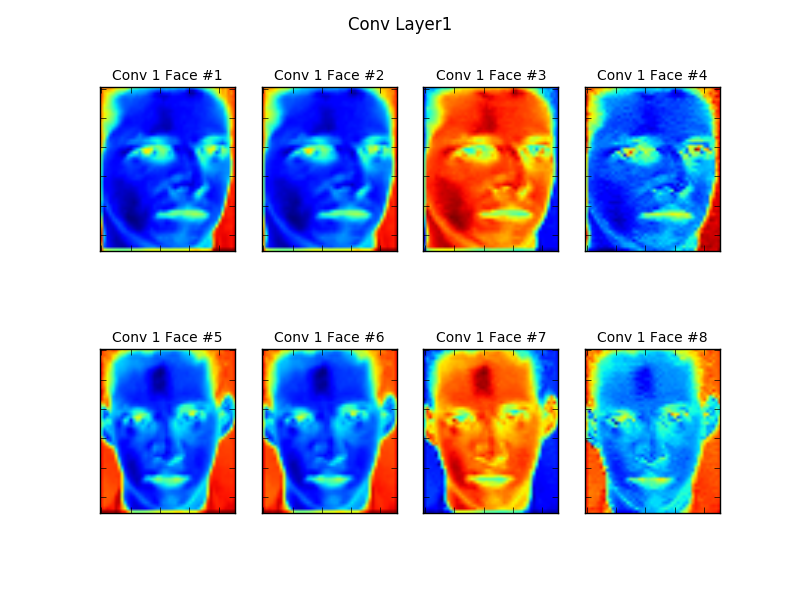
\includegraphics[width=0.65\linewidth]{../image/conv1.png}
\end{center}
使用了一个训练好的,正确率在$99\%$的卷积网络的参数,第一层卷积不同深度的feature mapping
\end{frame}
%------------------------------------------------------------
\begin{frame}
\frametitle{Keras实验:模型}
一个简单的CNN:\\
\begin{center}
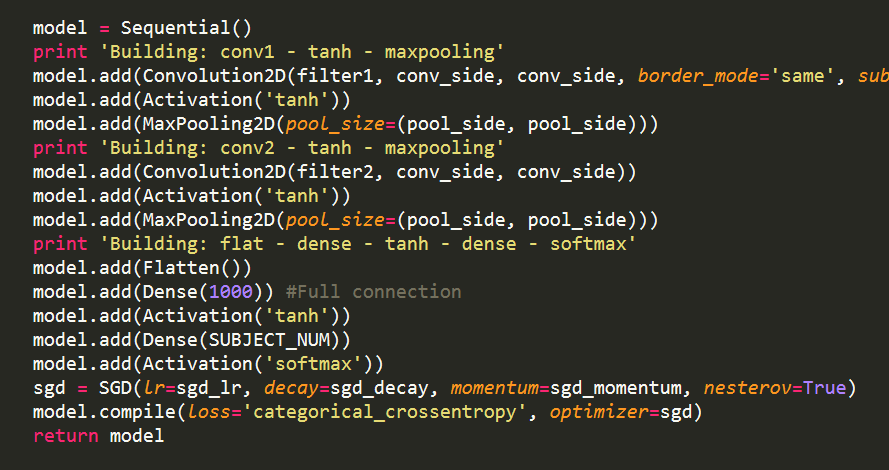
\includegraphics[width=1\linewidth]{./fig13.png}
\end{center}
\end{frame}
%------------------------------------------------------------
\begin{frame}
\frametitle{除了卷积以外还应该做什么}
max pooling:\\
\begin{center}
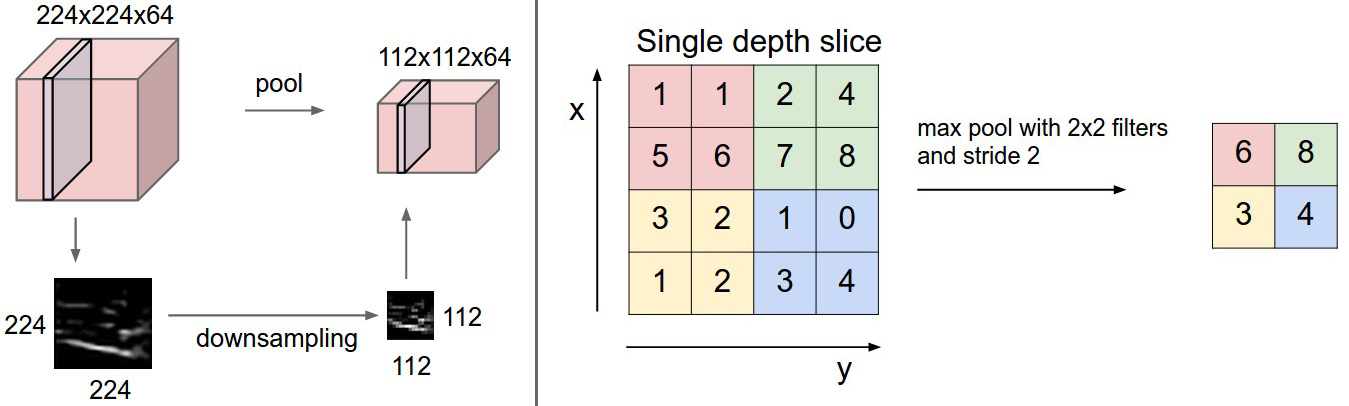
\includegraphics[width=0.8\linewidth]{./fig14.jpg}
\end{center}
对于一张合理的图像而言,临近点之间具有某种“连续性”\\
在某种意义上类似于“积分中值定理”:average pooling, max pooling
\end{frame}
%------------------------------------------------------------
\begin{frame}
\frametitle{为什么要做pooling}
Pooling的时候,“随意地”丢弃了很多特征图中的信息,所以可以对抗过拟合\\
如果用同样的方法去理解卷积filter呢?\\
或许,卷积filter可以看做一种更加精细的“积分中值定理”(实际上数学上的卷积就是这样的积分)\\
卷积filter+非线性和Pooling经常成对出现\\
 
\end{frame}
%------------------------------------------------------------
\begin{frame}
\frametitle{Keras实验: Max Pooling}
\begin{center}
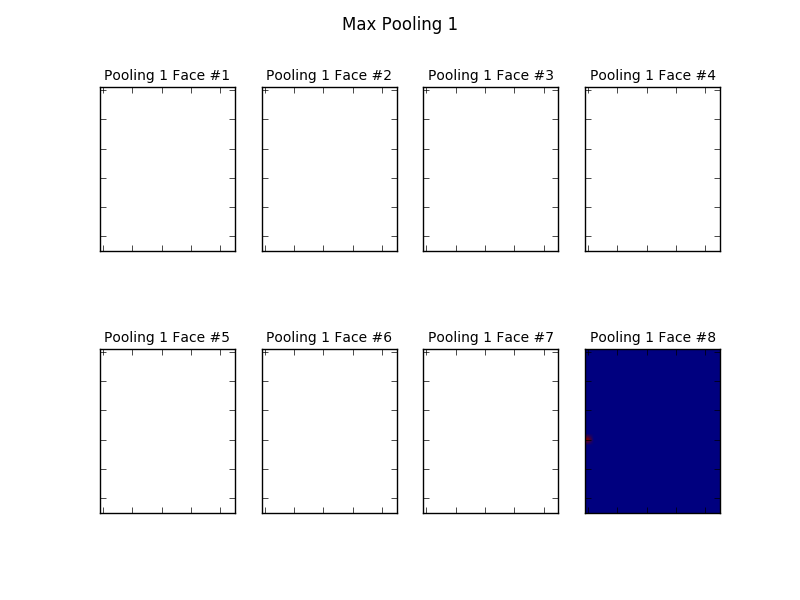
\includegraphics[width=0.65\linewidth]{../image/pool1.png}\\
???
\end{center}
\end{frame}
%------------------------------------------------------------
\begin{frame}
\frametitle{Keras实验: 第二层卷积}
\begin{center}
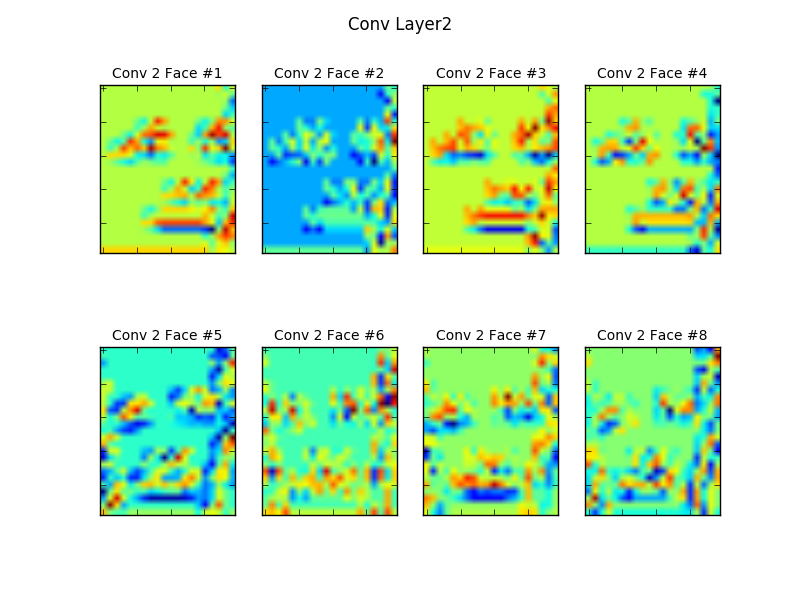
\includegraphics[width=0.65\linewidth]{../image/conv2.png}
\end{center}
可以看到,图片已经丢失了大部分信息\\
但是最主要的特征:眼睛、鼻子、嘴巴被保留了
\end{frame}
%------------------------------------------------------------
\begin{frame}
\frametitle{Keras实验: 第二层Pooling}
\begin{center}
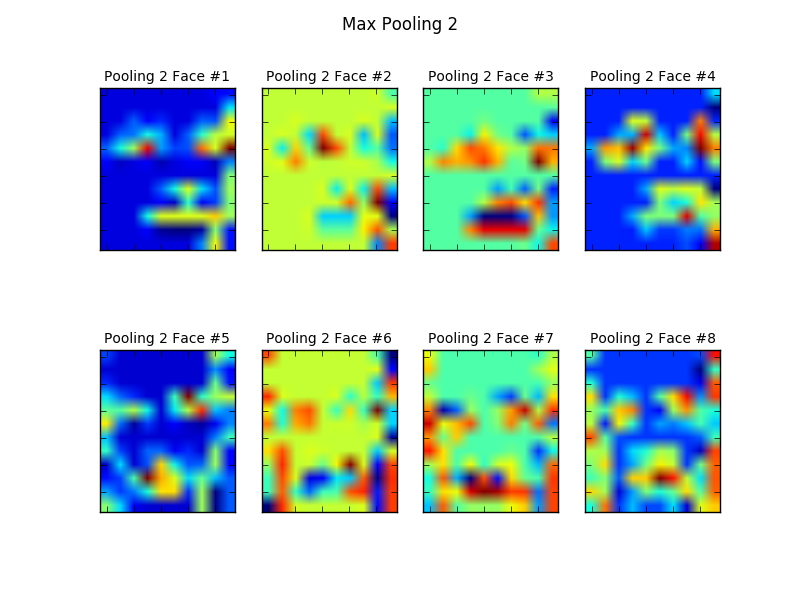
\includegraphics[width=0.65\linewidth]{../image/pool2.png}
\end{center}
更加抽象,但是网络已经抓取到了最具有特征的人脸五官信息\\
此时再做全连接网络的分类器,计算代价降低了很多
\end{frame}
%------------------------------------------------------------
\begin{frame}
\frametitle{影响结果的各种参数}
大家都熟知,所以不想讲太多\\
比如网络层数,层数越高,之前图片的信息“密度”越高,越从“局部感知”走向“全局感知”\\
我主要想讲的就是之前的原理
\end{frame}
%------------------------------------------------------------
\section{主成分分析}
\begin{frame}
\frametitle{PCA是如何想到的……}
\begin{center}
PCA是一个很棒的降维方法!\\
\end{center}
\bigskip
图片是维度特别高的输入,所以之前我们用CNN去抓取特征。\\
\begin{center}
在某些情况下,直接用PCA得到最重要的方向!
\end{center}
\end{frame}
%------------------------------------------------------------
\begin{frame}
\frametitle{PCA的前世今生}
源自1901年的统计学家:Karl Pearson\\
\bigskip
PCA的本质是找到高维空间上,对方差影响最大的数据方向\\
这样就能够权衡数据损失与空间维度!\\
\bigskip
数学上,PCA是特征分析多元统计分布的最简单的方法\\
现在,在复杂数据,比如人脸识别中非常有用
\end{frame}
%------------------------------------------------------------
\begin{frame}
\frametitle{一个简单的图示}
\begin{center}
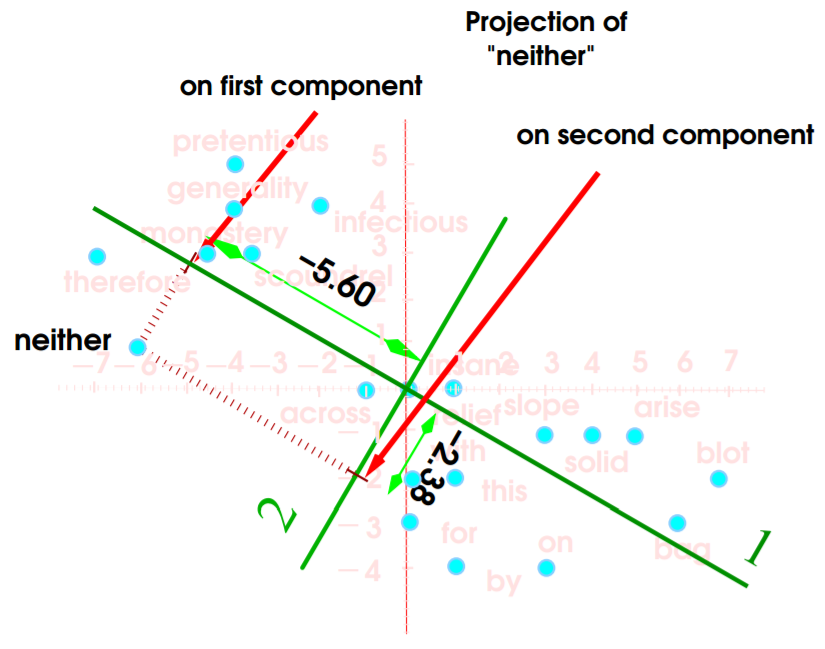
\includegraphics[width=0.8\linewidth]{fig19.png}
\\
得到了两个最重要的正交的方向
\end{center}
\end{frame}
%------------------------------------------------------------
\begin{frame}
\frametitle{优雅的数学推理}
为什么之前那两个方向是最重要的?\\
\bigskip
人脸$\mathbf{X} = \{\mathbf{x_1}, \mathbf{x_2}, \cdots, \mathbf{x_n} \} \in \mathbb{R}^{n \times d}$\\
\[ \mathbf{x_0} \in \mathbb{R}^{d} \]
希望它能最好地代表这些脸,或者说:与所有样本之间的距离的平方和越小越好:
\[ J_0(\mathbf{x_0}) = \sum_{k = 0}^n || \mathbf{x_0} - \mathbf{x_k} ||^2 \]
\end{frame}
%------------------------------------------------------------
\begin{frame}
\frametitle{优雅的数学推理}
拆开目标函数:
\[ J_0(\mathbf{x_0}) = \sum_{k = 1}^n || (\mathbf{x_0} - \mu ) - ( \mathbf{x_k} - \mu ) ||^2 \]

\[  = n\cdot || \mathbf{x_0} - \mathbf{\mu} ||^2 + \sum_{k = 0}^n || \mathbf{x_k} - \mathbf{\mu} ||^2  - 2 \cdot ||\mathbf{x_0} - \mathbf{\mu} || \cdot  \sum_{k = 0}^n ( \mathbf{x_k} - \mathbf{\mu} ) \]
\[  = n \cdot || \mathbf{x_0} - \mathbf{\mu} ||^2 + \sum_{k = 0}^n || \mathbf{x_k} - \mathbf{\mu} ||^2  \]
右边一项并不依赖于$\mathbf{x_0}$是常量,所以左边一项取均值$\mu$时目标函数取极小值
\end{frame}
%------------------------------------------------------------
\begin{frame}
\frametitle{优雅的数学推理}
这是否意味着就应该用均值$\mu$代表所有的人脸?\\
这样的观点基于这样一种看法,样本均值是数据的一种零维表达:\\
\[ \mu \in \mathbb{R}^0 \]
所以当我们用样本均值来降维的时候,降维降得过头了。所以现在考虑降到一维的情况,也就是将样本点投影到一条经过均值点的直线上,让这根直线上的投影点来代表全体数据点:
\[ \mathbf{x} = \mathbf{\mu} + a \cdot \mathbf{e} \]
在这里,标量$a$反应了投影点对均值的偏离程度,$\mathbf{e}$是单位方向向量
\end{frame}
%------------------------------------------------------------
\begin{frame}
\frametitle{优雅的数学推理}
现在,我们希望最小化投影点和实际点之间的差异:
\[ ||(\mathbf{\mu} + a_k \cdot \mathbf{e}) - \mathbf{x_k}|| \]
所以构造平方误差函数:\\
\[ J_1(a_1, \cdots, a_n, \mathbf{e}) = \sum_{k=1}^n ||(\mathbf{\mu} + a_k \cdot \mathbf{e}) - \mathbf{x_k}||^2  \]
\end{frame}
%------------------------------------------------------------
\begin{frame}
\frametitle{优雅的数学推理}
展开处理:
\[ J_1 = \sum_{k=1}^n a_k^2 - 2\sum_{k=1}^n a_k \mathbf{e^T}(\mathbf{x_k - \mu}) + \sum_{k=1}^n ||\mathbf{x_k - \mu}||^2 \]
这样就可以对$a_k$求偏导:\\
\[ \frac{\partial J_1}{\partial a_k} = 2a_k - 2\mathbf{e^T}(\mathbf{x_k - \mu}) = 0 \Rightarrow a_k = \mathbf{e^T}(\mathbf{x_k - \mu}) \]
\end{frame}
%------------------------------------------------------------
\begin{frame}
\frametitle{优雅的数学推理}
从几何上讲,这告诉我们向量$\mathbf{x_k}$只要向直线$\mathbf{e}$做垂直投影,就能得到最小方差。\\
\bigskip
接下来的问题是:如何找到直线$\mathbf{e}$的最优方向?\\
\begin{center}
散布矩阵
\end{center}
\[ \mathbf{S} = \sum_{k=1}^n (\mathbf{x_k - \mu})(\mathbf{x_k - \mu})^T \]
协方差矩阵的$n-1$倍
\end{frame}
%------------------------------------------------------------
\begin{frame}
\frametitle{优雅的数学推理}
用散布矩阵来描述目标函数:
\[ J_1(\mathbf{e}) = -\mathbf{e^TSe} + \sum_{k=1}^n ||\mathbf{x_k - \mu}||^2 \]
用Lagrange乘子法求$||\mathbf{e}||=1$的条件极值:
\[ u = -\mathbf{e^TSe} + \lambda \left( \mathbf{e^Te} - 1 \right) \]
\end{frame}
%------------------------------------------------------------
\begin{frame}
\frametitle{优雅的数学推理}
对$\mathbf{e}$求偏导:
\[ \frac{\partial u}{\partial \mathbf{e}} = 2\mathbf{Se} - 2\lambda\mathbf{e} = 0 \]
\[ \Rightarrow  \mathbf{Se} = \lambda\mathbf{e} \]
所以它一定是特征向量!\\
要让$\mathbf{e^TSe} = \lambda\mathbf{e^Te} = \lambda$最大\\
就要选取散布矩阵最大的特征值所对应的特征向量作为方向向量
\end{frame}
%------------------------------------------------------------
\begin{frame}
\frametitle{优雅的数学推理}
如果映射到高维空间$d'$呢?
\[ \mathbf{x = \mu} + \sum_{i=1}^{d'} a_i \mathbf{e_i} \]
取散布矩阵前$d'$个最大的特征值所对应的特征向量就行了\\
\bigskip
另外,散布矩阵
\[ \mathbf{S} = \sum_{k=1}^n (\mathbf{x_k - \mu})(\mathbf{x_k - \mu})^T \]
实对称,所以这些特征向量相互正交
\end{frame}
%------------------------------------------------------------
\begin{frame}
\frametitle{numpy实验}
还是用AT\&T的400张人脸灰度图像\\
因为数据集简单,所以虽然是简单模型,效果也很好,正确率在$99\%$左右
\end{frame}
%------------------------------------------------------------
\begin{frame}
\frametitle{numpy实验}
\begin{algorithm}[H]
\SetAlgoLined
$\mathbf{W}, \mu = \mathcal{PCA}(\mathbf{X})$\;
\For{$x_i \in \mathbf{X}$}{
	$\mathbf{P} \oplus \mathfrak{Projection}(\mathbf{W}, x_i, \mu)$\;
}
$\mathbf{Q} = \mathfrak{Projection}(W, x_i, \mu)$\;
\For{$i \in len(\mathbf{P})$}{
	$dist = ||\mathbf{P}[i], \mathbf{Q}||$\;
	\If{$dist <  dist_{min}$}{
		$dist_{min} = dist$\;
		$class_{min} = y_i$\;
	}
}
\caption{Prediction Algorithm of PCA}
\end{algorithm}
\end{frame}
%------------------------------------------------------------
\begin{frame}
\frametitle{numpy实验: 维度}
中间的结果也比较有趣,下图是一张脸在不同数量的特征向量上投影的结果:
\begin{center}
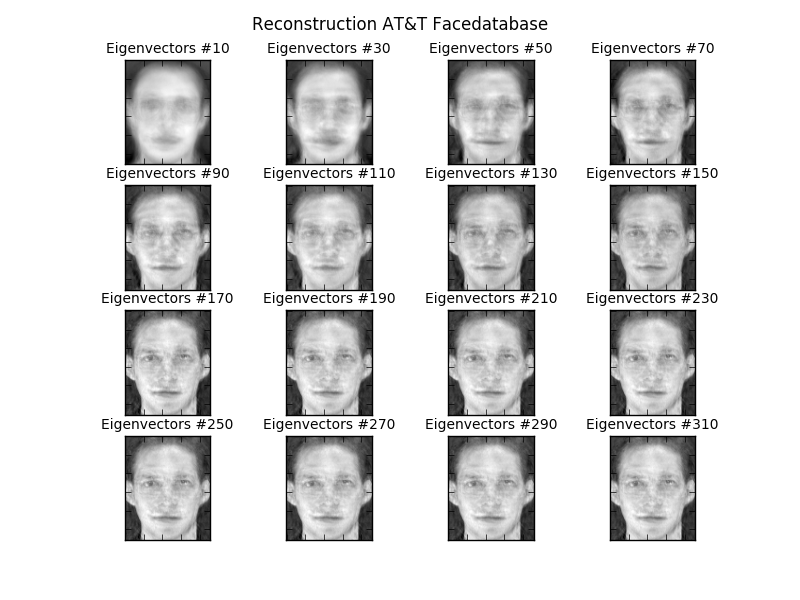
\includegraphics[width=0.6\linewidth]{../image/eigenvectors.png}
\end{center}
PCA投影的维度越高当然越接近原图
\end{frame}
%------------------------------------------------------------
\begin{frame}
\frametitle{numpy实验: Eigen Face}
从整个训练集中得到特征向量的矩阵$\mathbf{M} \in \mathbb{R}^{(H \cdot W) \times d'}$\\
取16个特征向量,归一化到$[0,255]$,还原成图片:
\begin{center}
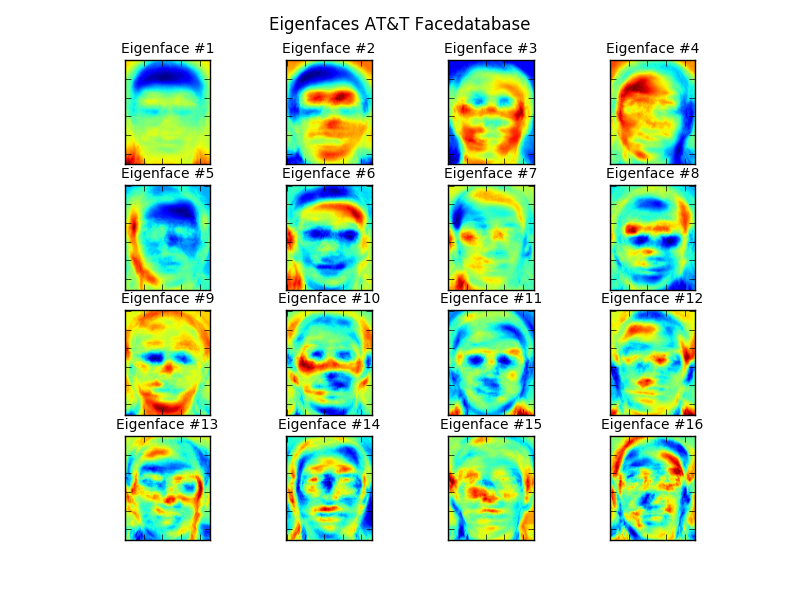
\includegraphics[width=0.65\linewidth]{../image/eigenfaces.png}
\end{center}
\end{frame}
%------------------------------------------------------------
\section{既成熟又不成熟的……}
\begin{frame}
\frametitle{其他方法的一点简单介绍}
\begin{itemize}
\item 古老的几何方法\\
计算眼耳鼻等面部特征之间的几何关系,在一个20人数据库上识别率为$45\% \sim 75\%$\\
\item 隐Markov模型\\
在垂直和水平方向(因为人脸会有稳定的结构)上,使用2维离散余弦变换系数作为特征……\\
\item 除了PCA, CNN之外的统计模型\\
Fisher判别法
\end{itemize}
\end{frame}
%------------------------------------------------------------
\begin{frame}
\frametitle{更复杂的课题}
\begin{itemize}
\item 光照变化\\
光照变化带来巨大的灰度相对分布,所以光照引起的变化甚至可能大过个体差异。\\
寻找不受光照影响的表达方式;改进现有算法(丢弃光照主成分);或者合成全面的人脸模型
\item 姿态变化\\
用2维投影线性组合重构3维对象的构想(流形)
\end{itemize}
\end{frame}
%------------------------------------------------------------
\begin{frame}
\frametitle{光照变化实验}
使用了Yale的扩展人脸数据集:
\begin{center}
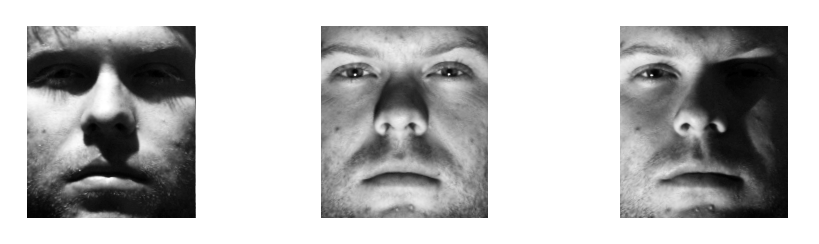
\includegraphics[width=1\linewidth]{./fig25.png}
\end{center}
具有光照变化
\end{frame}
%------------------------------------------------------------
\begin{frame}
\frametitle{光照变化实验: PCA的表现}
\begin{center}
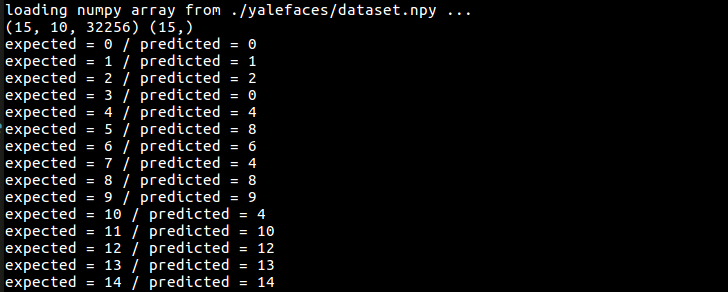
\includegraphics[width=1\linewidth]{./fig26.png}
\end{center}
明显比AT\&T数据集的表现要差一点。在AT\&T数据集上的识别率高达$99\%$,在具有光照变化的Yale数据集上降到了$66\%$
\end{frame}
%------------------------------------------------------------
\begin{frame}
\frametitle{光照变化实验: PCA的表现}
将PCA的特征脸抽取出来
\begin{center}
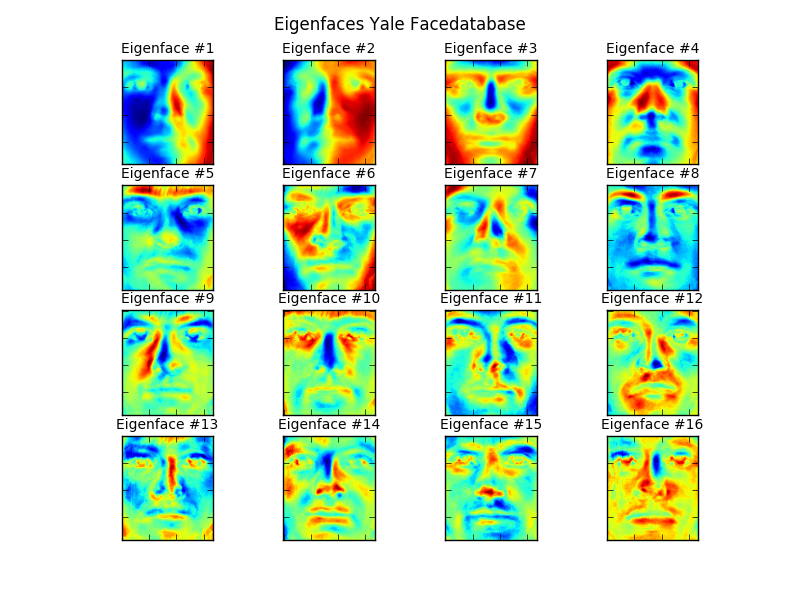
\includegraphics[width=0.65\linewidth]{../image/eigenfacesYale.png}
\end{center}
明显可以看到前几个特征向量收到光照的影响
\end{frame}
%------------------------------------------------------------
\begin{frame}
\frametitle{光照变化实验: CNN的表现}
CNN的表现要好很多,基本上依然维持在全部正确识别的水平
\begin{center}
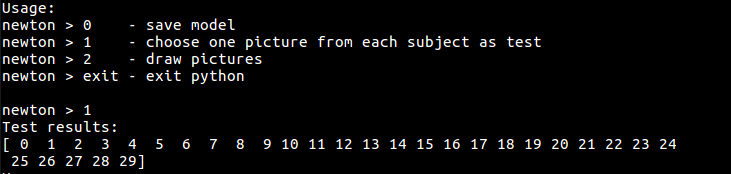
\includegraphics[width=1\linewidth]{./fig27.png}
\end{center}
这里两个模型都没有进行调整,所以PCA可能包含了具有光照效果的特征向量,导致识别率降低\\
可以看到,CNN对光照变化是比较不敏感的\\
这可能得益于CNN在每层的抽象上过滤了光照信息
\end{frame}
%------------------------------------------------------------
\begin{frame}
\frametitle{更复杂的应用场景}
针对性的人脸识别效果很好,但是更宽泛稳健的人脸识别系统还没有完善好\\
\bigskip
非常难以解决的问题是,当一个人戴上口罩、墨镜的时候,他自己的差异甚至大过与其他人之间的差异\\
\bigskip
要建立完善的人脸识别系统,图像的预处理占据了极大的比重
\end{frame}
%------------------------------------------------------------
\begin{frame}
\frametitle{参考资料}
\begin{itemize}
\item Stanford, CS231n, Computer Vision\\
\item github.com/bytefish/facerecognition guide\\
\item Keras, https://keras.io/
\item FBI, https://www.fbi.gov
\item AT\&T数据集\\
\item Yale数据集\\
\end{itemize}
\end{frame}
%------------------------------------------------------------
\end{document}